\scanpage{3}
\mspage{1}
\uline{Sur certains anneaux gradués}

\inserted{Soit $k$ anneau (\unsure{commut|comm}) fixé.}

1. \unsure{Soit|Soient} \deleted{$k$ un anneau,} $M^*$ un $k$-module gradué\inserted{\figure{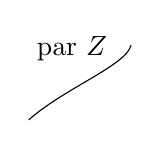
\begin{tikzpicture}[x=1cm,y=1cm]\node at (0,.35) {par $\mathbb Z$};\draw (-.55,-.55) .. controls (-.1,-.15) and (.7,.15) .. (.75,.4);\end{tikzpicture}}}, \inserted{\figure{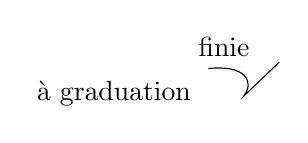
\begin{tikzpicture}[x=1cm,y=1cm]\node at (0,.05) {à graduation};\node at (1.4,.65) {finie};\draw (1.2,.37) .. controls (1.65,.42) and (1.8,.22) .. (1.65,.02)--(2.1,.45);\end{tikzpicture}}}, $\mathcal E^*$ une \deleted{algèbre graduée}\inserted{\figure{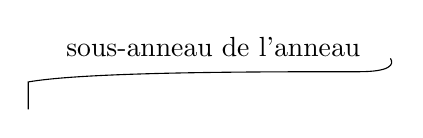
\begin{tikzpicture}[x=1cm,y=1cm]\node at (0,.35) {sous-anneau de l'anneau};\draw (-2.35,-.45)--(-2.35,-.1) .. controls (-1.6,.03) and (.6,.03) .. (1.85,.03) .. controls (2.25,.03) and (2.3,.12) .. (2.25,.2);\end{tikzpicture}}} d'endomorphismes \inserted{\figure{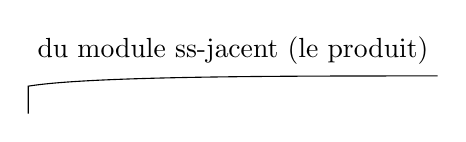
\begin{tikzpicture}[x=1cm,y=1cm]\node at (0,.35) {du module ss-jacent (le produit)};\draw (-2.6,-.45)--(-2.6,-.1) .. controls (-1.8,.03) and (.7,.03) .. (2.6,.03);\end{tikzpicture}}} de $M^*$. On désigne par $\pi_i$ la projection canonique de $M^*$ sur $M^i$. \deleted{et} On suppose que l'on a :
\[
\pi_i\in\mathcal E^*\quad\text{pour tout }i
\tag{1.2}
\]
Cela implique que $\mathcal E^*$ est une \uline{sous-}\deleted{\uline{algèbre}}\inserted{anneau} graduée de l'algèbre graduée \deleted{des} $\operatorname{End}(M^*)$ [dont la graduation est définie, si $\nu\in\mathbb Z$, par
\[
\operatorname{End}^{(\nu)}(M)=\sum\operatorname{Hom}(M^i,M^{i+\nu})
\]
ou de façon équivalente
\[
\operatorname{End}^{(\nu)}(M)=\sum_i\pi_{i+\nu}\operatorname{End}(M^*)\pi_i,
\]
la composante homogène de degré $\nu$ d'un endomorphisme $u$ de $M^*$ étant
\[
\deleted{\mathrm{gr}}\quad\operatorname{pr}_{\nu}(u)=\sum_i\pi_{i+\nu}u\pi_i.
\]
La graduation de $\mathcal E^*$ est définie \inserted{\figure{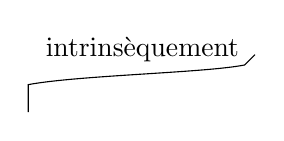
\begin{tikzpicture}[x=1cm,y=1cm]\node at (0,.35) {intrinsèquement};\draw (-1.45,-.45)--(-1.45,-.1) .. controls (-.8,.02) and (.8,.05) .. (1.3,.15)--(1.43,.28);\end{tikzpicture}}}, en termes de la \deleted{par} donnée des $\pi_i$, par
\[
\left\{\begin{aligned}
\text{\textcircled{a}}\quad&\boxed{\mathcal E^{(\nu)}=\sum_i\pi_{i+\nu}\mathcal E^*\pi_i}\,,\\
\text{\textcircled{b}}\quad&\operatorname{pr}_{\nu}^{\mathcal E}u=\sum_i\pi_{i+\nu}u\pi_i
\end{aligned}\right.
\tag{1.3}
\]
\margin{et $(1.4.)\quad u\in\mathcal E^{(\nu)}\Longleftrightarrow u\pi_i=\pi_{i+\nu}u$ pour tt $i$\par
$\deleted{\unsure{\Longleftrightarrow u=\pi_{i+\nu}u\pi_i}}$}
\margin{\figure{\begin{tikzpicture}[x=1cm,y=1cm]
\node[anchor=west] at (9.8,1.7) {Noter les relations};
\node[anchor=west] at (.2,.8) {$(1.1)$};
\node[anchor=west] at (.2,.25) {\deleted{Notons}};
\node[anchor=west] at (2.1,.55) {$\left\{\begin{aligned}\pi_i^2&=\pi_i\\\pi_i\pi_j&=0\quad\text{si }i\neq j\\\sum\pi_i&=1\end{aligned}\right.$};
\draw[draw=brown!60!black] (.25,1.35) .. controls (-.1,1.15) and (-.35,.25) .. (.05,.05) .. controls (2,-.4) and (8,-.2) .. (11.5,.1) .. controls (13.8,.2) and (14.2,1.7) .. (13.2,2.0) .. controls (11.5,2.15) and (6.8,1.2) .. (.65,1.32);
\draw[draw=brown!60!black] (.3,1.15)--(.1,.65);
\draw[draw=brown!60!black] (.1,.6) circle (.055);
\end{tikzpicture}}}

2. Soit $\mathcal E^*$ une \deleted{$k$-algèbre}\inserted{anneau} graduée, et soient $\pi_i$ ($i\in\mathbb Z$) des éléments de $\mathcal E$, \inserted{\figure{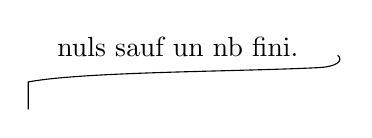
\begin{tikzpicture}[x=1cm,y=1cm]\node at (0,.35) {nuls sauf un nb fini.};\draw (-1.9,-.45)--(-1.9,-.1) .. controls (-1.2,.03) and (.7,.03) .. (1.75,.08) .. controls (2.05,.09) and (2.1,.18) .. (2.03,.24);\end{tikzpicture}}} A quelles conditions les formules $(1.3)$ définissent-elles
\mspage{2}
